\documentclass{article}

    \usepackage{fancyhdr}
    \usepackage{extramarks}
    \usepackage{amsmath}
    \usepackage{amsthm}
    \usepackage{amsfonts}
    \usepackage{tikz}
    \usepackage{amssymb}
    \usepackage{subcaption}
    \usepackage{blkarray}
    \usetikzlibrary{arrows, automata}
    \usepackage{forest}
    
    \usetikzlibrary{trees}
    


    \usetikzlibrary{decorations.markings}
    \tikzstyle{vertex}=[circle, draw, inner sep=0pt, minimum size=6pt]
    \newcommand{\vertex}{\node[vertex]}

    
    \usepackage{amsmath}
    \usepackage{algorithm}
    \usepackage[noend]{algpseudocode}
    \usepackage[utf8]{inputenc}
    \usepackage{enumerate}
    \usepackage{geometry}
    \usepackage{mathtools}
    \usepackage{parskip}
    \usepackage{xifthen, xparse}
    
    \algdef{SE}[SUBALG]{Indent}{EndIndent}{}{\algorithmicend\ }%
    \algtext*{Indent}
    \algtext*{EndIndent}
    
    
    
    \usetikzlibrary{automata,positioning}
    
    %
    % Basic Document Settings
    %
    
    \topmargin=-0.45in
    \evensidemargin=0in
    \oddsidemargin=0in
    \textwidth=6.5in
    \textheight=9.0in
    \headsep=0.25in
    
    \linespread{1.1}
    
    \pagestyle{fancy}
    \lhead{\hmwkAuthorName}
    \chead{\hmwkClass\ \hmwkTitle}
    \rhead{\firstxmark}
    \lfoot{\lastxmark}
    \cfoot{\thepage}
    
    \renewcommand\headrulewidth{0.4pt}
    \renewcommand\footrulewidth{0.4pt}
    
    \setlength\parindent{0pt}
    
    %
    % Create Problem Sections
    %
    
    \newcommand{\enterProblemHeader}[1]{
        \nobreak\extramarks{}{Problem \arabic{#1} continued on next page\ldots}\nobreak{}
        \nobreak\extramarks{Problem \arabic{#1} (continued)}{Problem \arabic{#1} continued on next page\ldots}\nobreak{}
    }
    
    \newcommand{\exitProblemHeader}[1]{
        \nobreak\extramarks{Problem \arabic{#1} (continued)}{Problem \arabic{#1} continued on next page\ldots}\nobreak{}
        \stepcounter{#1}
        \nobreak\extramarks{Problem \arabic{#1}}{}\nobreak{}
    }
    
    \newcommand\rowop[1]{\scriptstyle\smash{\xrightarrow[\vphantom{#1}]{\mkern-4mu#1\mkern-4mu}}}
    
    \DeclareDocumentCommand\converttorows%
    {>{\SplitList{,}}m}%
    {\ProcessList{#1}{\converttorow}}
    \NewDocumentCommand{\converttorow}{m}
    {\ifthenelse{\isempty{#1}}{}{\rowop{#1}}\\}
    
    \DeclareDocumentCommand \rowops{m}
    {\;
     \begin{matrix}
    \converttorows {#1}
     \end{matrix}
     \; }
    
    \setcounter{secnumdepth}{0}
    \newcounter{partCounter}
    \newcounter{homeworkProblemCounter}
    \setcounter{homeworkProblemCounter}{1}
    \nobreak\extramarks{Problem \arabic{homeworkProblemCounter}}{}\nobreak{}
    
    %
    % Homework Problem Environment
    %
    % This environment takes an optional argument. When given, it will adjust the
    % problem counter. This is useful for when the problems given for your
    % assignment aren't sequential. See the last 3 problems of this template for an
    % example.
    %
    \newenvironment{homeworkProblem}[1][-1]{
        \ifnum#1>0
            \setcounter{homeworkProblemCounter}{#1}
        \fi
        \section{Problem \arabic{homeworkProblemCounter}}
        \setcounter{partCounter}{1}
        \enterProblemHeader{homeworkProblemCounter}
    }{
        \exitProblemHeader{homeworkProblemCounter}
    }
    
    %
    % Homework Details
    %   - Title
    %   - Due date
    %   - Class
    %   - Section/Time
    %   - Instructor
    %   - Author
    %
    
    \newcommand{\hmwkTitle}{SOFTENG250 Assignment \#3}
    \newcommand{\hmwkClass}{D.S. and Algorithms}
    \newcommand{\hmwkAuthorName}{\textbf{Nisarag Bhatt}}
    \newcommand{\idnumber}{945034068}
    \newcommand{\upi}{nbha702}
    
    %
    % Title Page
    %
    
    \title{
        \vspace{2in}
        \textmd{\textbf{\hmwkClass:\ \hmwkTitle}}\\
        \vspace{3in}
    }
    
    \author{\hmwkAuthorName}
    \date{}
    
    \renewcommand{\part}[1]{\textbf{\large Part \Alph{partCounter}}\stepcounter{partCounter}\\}
    
    %
    % Various Helper Commands
    %
    
    % Useful for algorithms
    \newcommand{\alg}[1]{\textsc{\bfseries \footnotesize #1}}
    
    % For derivatives
    \newcommand{\deriv}[1]{\frac{\mathrm{d}}{\mathrm{d}x} (#1)}
    
    % For partial derivatives
    \newcommand{\pderiv}[2]{\frac{\partial}{\partial #1} (#2)}
    
    % Integral dx
    \newcommand{\dx}{\mathrm{d}x}
    
    % Alias for the Solution section header
    \newcommand{\solution}{\textbf{\large Solution}}
    
    % Probability commands: Expectation, Variance, Covariance, Bias
    \newcommand{\E}{\mathrm{E}}
    \newcommand{\Var}{\mathrm{Var}}
    \newcommand{\Cov}{\mathrm{Cov}}
    \newcommand{\Bias}{\mathrm{Bias}}
    
    \begin{document}
    
    
    
    \pagebreak
    
    \begin{homeworkProblem}
        \textbf{Question:} Solve Exercises 1-4 and Exercise 6 from LN4.pdf.
        
        \textbf{Excercise 1:} Which vertices of the graph in Figure 1 are connected with each other and which vertices are not?

        \textbf{Solution:}
        $$ \text{Subgraphs} = \{G_1 = \{2,4,7,8\} , G_2 = \{0,1,3,5\}, G_3 = \{6,9\} \}$$

        $G_1,G_2,G_3$ are all connected sub-graphs of $G$. Since in all these sub-graphs all pairs of vertices in these sub-graphs are connected
        with each other we have that  vertices of $G_1$ are not connected with the vertices $G_2$ and $G_3$ respectively.

        \textbf{Excercise 2:} Consider the undirected graph model of Facebook. Reason about if the graph is connected or not.

        \textbf{Solution:}

        On Facebook we can say people are \textit{vertices} and if two people are friends there is an undirected \textit{edge} between them.

        Since it is impossible that every person in the graph is friends with every other person on Facebook, this suggests that the graph model is not connected.

        \textbf{Excercise 3:} Prove \begin{enumerate}
            \item Every vertex $v$ is of the graph is connected to itself
            \item If a vertex $v$ is connected to a vertex $u$ then $u$ is connected to $v$.
            \item If a vertex $v$ is connected to $u$ and $u$ is connected to $w$ then $v$ is connected to $w$.
        \end{enumerate}

        \textbf{Solution:}

        \begin{enumerate}
            \item In a connected graph, there are no unreachable vertices, every vertex must be connected to every other vertex. Therefore there must be a path travelling from vertex $v$ to itself. In the case where only $1$ vertex is in the graph, the vertex will be connected to itself in a path length = $0$.
            \item In a connected graph, there are no unreachable vertices, every vertex must be connected to every other vertex. If a path exists from vertex $u$ to vertex $v$, a path must also exists from vertex $v$ to vertex $u$ as the edges of a graph are undirected (travel in reverse using the same path).
            \item If vertex $v$ is connected to vertex $u$, it means a path also exists between the $2$ vertices. Similarly if vertex $u$ is connected to vertex $w$, a path exists from vertex $u$ to vertex $w$. Therefore, if we start at vertex $v$ and travel in the sequence of vertex $v$ to vertex u to vertex w, we find that a path exists from vertex v to vertex w (vertex $v$ is connected to vertex $w$).
        \end{enumerate}

        \textbf{Excercise 4:} Let $C(u)$ and $C(v)$ be two components of graphs $G$. Explain that either $C(u)=C(v)$ (that is, these two components coincide) or the
        components $C(u)$ and $C(v)$ have no vertices in common (written $C(u) \cap C(v) = \emptyset)$.

        \textbf{Solution:}

        If there are only $2$ components in the graph, all vertices within a single component are said to be connected and each of the components must either be connected or not connected at all. 

        If the components are connected, as a graph is undirected, the graph itself will be a single component. Therefore, a vertex will be connected to all other vertices, hence the component of vertex $v$ will be $C(v) = \{\text{all other vertices}\}$ and the component of vertex u will be $C(u) = \{\text{all other vertices}\}$ proving $C(v) = C(u)$.

        Alternatively, if they are not connected, it means any vertices in the component $C(v)$ will not be connected to any of the vertices in $C(u)$. Therefore vertices in $C(v)$ cannot be in $C(u)$ and this proves $C(u) \cap C(v)= \emptyset$.

        \textbf{Excercise 6:} Explain why a tree has $n$ nodes has exactly $n-1$ edges.

        \textbf{Solution:}

        Assume starting with a single vertex representing the root of the tree, for every new connected vertex that does not create a cycle (trees does not have any cycles). $1$ edge and the $1$ new vertex must be added on. Therefore, at the end of the tree (the leaves), there will be $1$ less edge than vertices as the starting vertex does not start with any edges.

        \textbf{We can also prove this by induction:}

        Let $v$ denote the terminal vertex (with degree $1$). (leaf)

        Base Case: For $n=1$, we have that there are $0$ edges. Which is true.

        Inductive Step: Let $n=k$ and assume true for $k$ (i.e. Assume that every tree with $k$ vertices has $k-1$ edges)

        Now let $T$ be a tree with $k+1$ vertices, now consider a tree $T'$ where $v$ (the terminal vertex) has been removed, since $T'$ has $k$ vertices it must have $k-1$ edges by induction. However
        $v$ is the terminal vertex with degree $1$, therefore $T$ has one more edge than $T'$ and this completes the proof.


    \end{homeworkProblem}
    
    \begin{homeworkProblem}
        \textbf{Question:} Draw three graphs $G_1$, $G_2$ and $G_3$ such that $(1)$ each graph has exactly $5$ vertices; $(2) G_1$
        has exactly $1$ component, $G_2$ has exactly $2$ components, and $G_3$ has exactly $3$ components.
        \begin{figure}[H]
            \centering
            \begin{subfigure}[b]{0.3\textwidth}
                \centering
                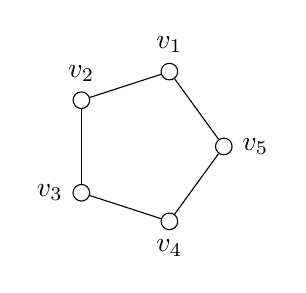
\begin{tikzpicture}
                    \vertex (v1) at (72:1) [label=above:$v_1$]{};
                    \vertex (v2) at (144:1) [label=above:$v_2$]{};
                    \vertex (v3) at (216:1) [label=left:$v_3$]{};
                    \vertex (v4) at (288:1) [label=below:$v_4$]{};
                    \vertex (v5) at (360:1) [label=right:$v_5$]{};
                    \path 
                        (v1) edge (v2) 
                        (v2) edge (v3)
                        (v3) edge (v4)
                        (v4) edge (v5)
                        (v5) edge (v1)
                    ;
                \end{tikzpicture}
                \caption{$G_1$}
                \label{fig:g2}
                \centering
            \end{subfigure}
            \centering
            \centering
            \begin{subfigure}[b]{0.3\textwidth}
                \centering
                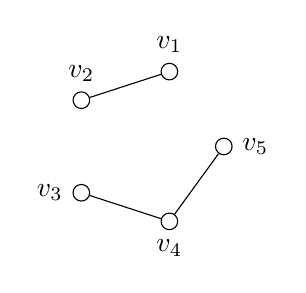
\begin{tikzpicture}
                    \vertex (v1) at (72:1) [label=above:$v_1$]{};
                    \vertex (v2) at (144:1) [label=above:$v_2$]{};
                    \vertex (v3) at (216:1) [label=left:$v_3$]{};
                    \vertex (v4) at (288:1) [label=below:$v_4$]{};
                    \vertex (v5) at (360:1) [label=right:$v_5$]{};
                    \path 
                        (v1) edge (v2)
                        (v3) edge (v4)
                        (v4) edge (v5)
                    ;
                \end{tikzpicture}
                \caption{$G_2$}
                \label{fig:g2}
                \centering
            \end{subfigure}
            \centering
            ~ %add desired spacing between images, e. g. ~, \quad, \qquad, \hfill etc. 
            %(or a blank line to force the subfigure onto a new line)
            \centering
            \begin{subfigure}[b]{0.3\textwidth}
                \centering
                \begin{tikzpicture}
                    \vertex (v1) at (72:1) [label=above:$v_1$]{};
                    \vertex (v2) at (144:1) [label=above:$v_2$]{};
                    \vertex (v3) at (216:1) [label=left:$v_3$]{};
                    \vertex (v4) at (288:1) [label=below:$v_4$]{};
                    \vertex (v5) at (360:1) [label=right:$v_5$]{};
                    \path 
                        (v1) edge (v2)
                        (v4) edge (v5)
                    ;
                \end{tikzpicture}
                \caption{$G_3$}
                \label{fig:g3}
                \centering
            \end{subfigure}
            \caption{Collection of Graphs}\label{fig:graphs}
            \centering
        \end{figure}
    \end{homeworkProblem}

    \begin{homeworkProblem}
        \textbf{Question:} Solve Exercises 1-5 in LN5.pdf

        \textbf{Excercise 1:} Construct two distinct BFS-trees for each of the following graphs: the wheel graph $W_5$ and the cube graph $\text{Cube}_3$.

        \textbf{Solution:}
        \begin{figure}[H]
            \centering
            \begin{subfigure}[b]{0.3\textwidth}
                \centering
                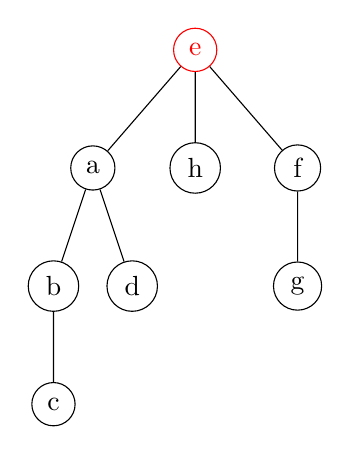
\begin{tikzpicture}[level distance=1.5cm,
                    level 1/.style={sibling distance=1.3cm},
                    level 2/.style={sibling distance=1cm}]
                    level 3/.style={sibling distance=0.8cm}]
                    \tikzstyle{every node}=[circle,draw]
                    
                    \node (Root) [red] {e}
        
                    child {
                        node {a}
                        child { 
                            node {b} 
                            child {node {c}} 
                        }
                        child { node {d} }
                    }
                    child {
                        node {h}
                    }
                    child {
                        node {f} 
                        child { node {g} }
                    };
                \end{tikzpicture}
                \caption{$\text{BFS}(\text{Cube}_3,e)$}
                \label{fig:g2}
                \centering
            \end{subfigure}
            \centering
            \centering
            \begin{subfigure}[b]{0.3\textwidth}
                \centering
                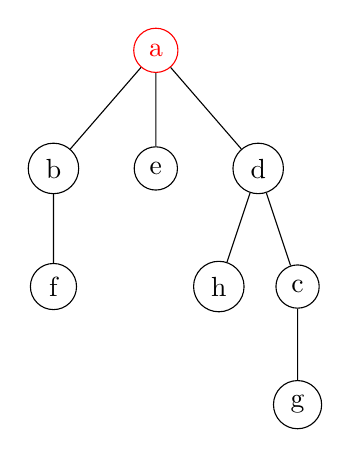
\begin{tikzpicture}[level distance=1.5cm,
                    level 1/.style={sibling distance=1.3cm},
                    level 2/.style={sibling distance=1cm}]
                    level 3/.style={sibling distance=0.8cm}]
                    \tikzstyle{every node}=[circle,draw]
                    
                    \node (Root) [red] {a}
        
                    child {
                        node {b} 
                        child { node {f} }
                    }
                    child {
                        node {e}
                    }
                    child {
                        node {d}
                        child { node {h} }
                        child { 
                            node {c} 
                            child {node {g}} 
                        }
                    };
                \end{tikzpicture}
                \caption{$\text{BFS}(\text{Cube}_3,a)$}
                \label{fig:g2}
                \centering
            \end{subfigure}
            \centering
            \caption{ BFS on $\text{Cube}_3$ }\label{fig:graphs}
            ~ %add desired spacing between images, e. g. ~, \quad, \qquad, \hfill etc. 
            %(or a blank line to force the subfigure onto a new line)

        \end{figure}

        \begin{figure}[H]
            \centering
            \begin{subfigure}[b]{0.3\textwidth}
                \centering
                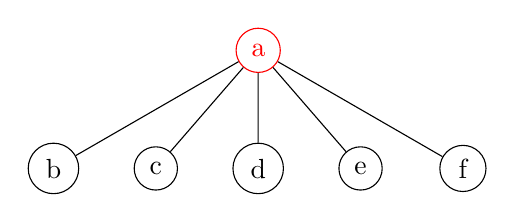
\begin{tikzpicture}[level distance=1.5cm,
                    level 1/.style={sibling distance=1.3cm},
                    level 2/.style={sibling distance=1cm}]
                    level 3/.style={sibling distance=0.8cm}]
                    \tikzstyle{every node}=[circle,draw]
                    \node (Root) [red] {a}
                    child {
                        node {b}
                    }
                    child {
                        node {c}
                    }
                    child {
                        node {d} 
                    }
                    child {
                        node {e} 
                    }
                    child {
                        node {f} 
                    };
                \end{tikzpicture}
                \caption{$\text{BFS}(W_5,a)$}
                \label{fig:g2}
                \centering
            \end{subfigure}
            \centering
            \centering
            \begin{subfigure}[b]{0.3\textwidth}
                \centering
                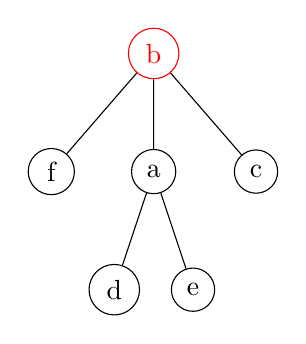
\begin{tikzpicture}[level distance=1.5cm,
                    level 1/.style={sibling distance=1.3cm},
                    level 2/.style={sibling distance=1cm}]
                    level 3/.style={sibling distance=0.8cm}]
                    \tikzstyle{every node}=[circle,draw]
                    \node (Root) [red] {b}
                    child {
                        node {f}
                    }
                    child {
                        node {a}
                        child { node {d} }
                        child { node {e} }
                    }
                    child {
                        node {c} 
                    };
                \end{tikzpicture}
                \caption{$\text{BFS}(W_5,b)$}
                \label{fig:g2}
                \centering
            \end{subfigure}
            \centering
            \caption{ BFS on wheel graph $W_5$}\label{fig:graphs}
            ~ %add desired spacing between images, e. g. ~, \quad, \qquad, \hfill etc. 
            %(or a blank line to force the subfigure onto a new line)

        \end{figure}

        \textbf{Excercise 2:} Let $x$ and $y$ be vertices of $G$ such that $x$ is in the layer $L_i$ and $y$ is in $L_j$. Show that
        if there is an edge in the graph $G$ between $x$ and $y$ then $i$ and $j$ differ at most by $1$.

        \textbf{Solution:}

        In the case, if $x$ is found first, then $x$ will be in layer $i$ (for $i<j$). 
        If an edge exists between $x$ and $y$, then $y$ must be in the following layer $j$ as it is a neighbour of $x$ (BFS finds all neighbours and put them in the next layer). Therefore, $i$ and $j$ will be separated by a distance of $1$. Alternatively, if $y$ is found first then the same logic applies as above. 
        
        In the case where both $x$ and $y$ are found at the same time, they will be in the same layer $(i=j)$ and the criteria, difference of at most $1$ is still valid.

        \textbf{Excercise 3:} What are the heights of the BFS-trees for the wheel graphs $W_n$

        \textbf{Solution:}

        Assume first layer is labelled as $L_0$

        We can consider two cases:

        If the middle vertex is the vertex representing the “root” of a tree. The tree will have a height of $1$ as the middle vertex is connected to all other vertices in the wheel (All other vertex will be in layer $1$ in the BFS algorithm).

        Alternatively, if any other vertex is used to represent the “root” of the tree. The tree will have a height of $2$ as in the $1st$ layer, BFS will reach the middle vertex as the middle vertex is connected to every other vertex in the wheel. 
        In the 2nd layer, the middle vertex will then able to have all other vertex which has not been reached to become a “child” of the middle vertex.

        \textbf{Excercise 4:} Prove that the height of any $BFS$-tree for graph $G$ starting at $x$ is smaller or equal to the heights
        of all $DFS$-trees for $G$ starting at $x$.

        \textbf{Solution:}

        Since BFS finds path using the fewest number of edges, the BFS depth of any vertex is at least as small as the DFS depth of the same vertex. Thus the DFS tree has a greater or equal depth.

        Alternatively use proof by contradiction:

        Assume the DFS tree is less in height than the BFS tree. Then the longest branch in DFS is shorter than the longest branch in BFS

        Let node $v$ be the leaf node of the DFS branch. If the height of the branch is $n$, then $v$ is reachable from $s$ (root node) by traversing $n$ edges. (Distance from $s$ to $v$ is $n$).

        BFS discovers nodes with nearest distance first. When BFS discovers v, distance to v is $m>n$. But all nodes with distance from root $< m$ have already been discovered. Therefore $v$ has already been discovered, thus contradiction.

        Therefore DFS creates tree of height $ \geq $ to that of BFS.

        \textbf{Excercise 5:} Describe adjacency matrix representations for complete graphs $K_n$, bipartite graphs $K_{n,m}$, wheel graphs, and cycle graphs $C_n$.

        \textbf{Solution:}

        Assume all the graphs are undirected.

        \begin{itemize}
            \item A complete graph $K_n$ will have an “$n$ by $n$” adjacency matrix with all elements as $1$ except the leading diagonal as 0 because a vertex cannot connect to itself in an undirected graph.
            \item A bipartite graph $K_{n,m}$ will have an “$n$ by $n$” zero matrix at the top left corner as all the vertex in the column $n$ cannot connect to itself. Similarly, the matrix will have an “$m$ by $m$” zero matrix at the bottom right corner as all the vertex in the column $m$ cannot connect to itself. The top right corner will contain an “$n$ by $m$” matrix containing information of how each of the vertex in the list $n$ is connected to each of the vertex in the list $m$. Finally, the bottom left corner will have the “$m$ by $n$” transpose matrix of the top right corner showing how each of the vertex in list $m$ is connected back to vertex in list $n$.
        $$ \therefore adj(K_{n,m}) = \begin{pmatrix}0_{n,n} & B_{n,m} \\ B^{T}_{m,n} & 0_{m,m} \end{pmatrix}$$
            \item The adjacency matrix of a cycle graph will have zeroes on the leading diagonal as a vertex cannot connect to itself. Assuming the labelling convention is “$1$ through to $n$” in a cyclic order. The matrix will have $1$'s right above and below the leading diagonal of zeroes. It will also have $1$'s in the top right and bottom left corner of the matrix as the vertex $n$ will be connected to vertex $1$ and reversely $1$ connected to $n$ as well. This makes each row and column of the matrix to have exactly $2$ ones.
            For example
        $$ adj(C_4) = \begin{pmatrix} 0 & 1 & 0 & 1 \\ 1 & 0 & 1 & 0 \\ 0 & 1 & 0 & 1 \\ 1 & 0 & 1 & 0\end{pmatrix}$$
                            
            \item The adjacency matrix of a wheel graph will have the following 3 conditions: 
                \begin{enumerate}
                    \item One of the row and one of the column must have all ones except the element on the leading diagonal of the matrix (middle matrix).
                    \item The leading diagonal must be all zeroes.
                    \item Each row and each column must have exactly 3 ones.
                \end{enumerate}

                We can also notice that the adjacency matrix of $W_n$ is quite similar to the $C_n$ since in the $W_n$ we have a middle terminal vertex where every outer vertex is connected to that one.

                For example consider:
            $$adj(W_4) = \begin{pmatrix} 0 & 1 & 0 & 1 & 1 \\ 1 & 0 & 1 & 0 & 1 \\ 0 & 1 & 0 & 1 & 1 \\ 1 & 0 & 1 & 0 & 1 \\ 1 & 1 & 1 & 1 & 0\end{pmatrix}$$
        \end{itemize}



    \end{homeworkProblem}

    \begin{homeworkProblem}
        \textbf{Question:} Fix $n > 0$ and $k > 0$. Draw a directed graph with $k \cdot n$ vertices such that the graph has
        exactly $n$ strongly connected components.

        \textbf{Solution:}

        \[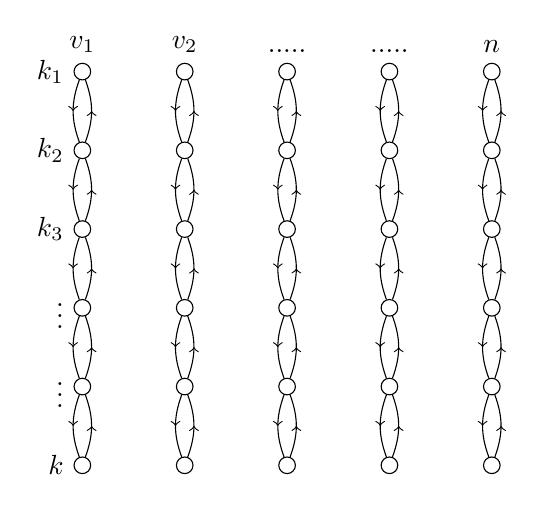
\begin{tikzpicture}[x=1.3cm, y=1cm,
            every edge/.style={
                draw,
                postaction={decorate,
                            decoration={markings,mark=at position 0.5 with {\arrow{>}}}
                           }
                }
        ]

            \vertex (v1) at (0,0) [label=above:$v_1$,label=left:$k_1$]{};
            \vertex (v6) at (0,-1) [label=left:$k_2$]{};
            \vertex (v7) at (0,-2) [label=left:$k_3$]{};
            \vertex (v8) at (0,-3) [label=left:$\vdots$]{};
            \vertex (v9) at (0,-4) [label=left:$\vdots$]{};
            \vertex (v10) at (0,-5) [label=left:$k$]{};

        
            \vertex (v2) at (1,0) [label=above:$v_2$]{};
            \vertex (v11) at (1,-1) [label=left:$$]{};
            \vertex (v15) at (1,-2) [label=left:$$]{};
            \vertex (v19) at (1,-3) [label=left:$$]{};
            \vertex (v23) at (1,-4) [label=left:$$]{};
            \vertex (v27) at (1,-5) [label=left:$$]{};

            \vertex (v3) at (2,0) [label=above:$.....$]{};
            \vertex (v12) at (2,-1) [label=left:$$]{};
            \vertex (v16) at (2,-2) [label=left:$$]{};
            \vertex (v20) at (2,-3) [label=left:$$]{};
            \vertex (v24) at (2,-4) [label=left:$$]{};
            \vertex (v28) at (2,-5) [label=left:$$]{};

            \vertex (v4) at (3,0) [label=above:$.....$]{};
            \vertex (v13) at (3,-1) [label=left:$$]{};
            \vertex (v17) at (3,-2) [label=left:$$]{};
            \vertex (v21) at (3,-3) [label=left:$$]{};
            \vertex (v25) at (3,-4) [label=left:$$]{};
            \vertex (v29) at (3,-5) [label=left:$$]{};

            \vertex (v5) at (4,0) [label=above:$n$]{};
            \vertex (v14) at (4,-1) [label=left:$$]{};
            \vertex (v18) at (4,-2) [label=left:$$]{};
            \vertex (v22) at (4,-3) [label=left:$$]{};
            \vertex (v26) at (4,-4) [label=left:$$]{};
            \vertex (v30) at (4,-5) [label=left:$$]{};

            \path
                (v1) edge[bend right=20] (v6)
                (v6) edge[bend right=20] (v7)
                (v7) edge[bend right=20] (v8)
                (v8) edge[bend right=20] (v9)
                (v9) edge[bend right=20] (v10)
                (v10) edge[bend right=20] (v9)
                (v9) edge[bend right=20] (v8)
                (v8) edge[bend right=20] (v7)
                (v7) edge[bend right=20] (v6)
                (v6) edge[bend right=20] (v1)

                (v2) edge[bend right=20] (v11)
                (v11) edge[bend right=20] (v15)
                (v15) edge[bend right=20] (v19)
                (v19) edge[bend right=20] (v23)
                (v23) edge[bend right=20] (v27)
                (v27) edge[bend right=20] (v23)
                (v23) edge[bend right=20] (v19)
                (v19) edge[bend right=20] (v15)
                (v15) edge[bend right=20] (v11)
                (v11) edge[bend right=20] (v2)

                (v3) edge[bend right=20] (v12)
                (v12) edge[bend right=20] (v16)
                (v16) edge[bend right=20] (v20)
                (v20) edge[bend right=20] (v24)
                (v24) edge[bend right=20] (v28)
                (v28) edge[bend right=20] (v24)
                (v24) edge[bend right=20] (v20)
                (v20) edge[bend right=20] (v16)
                (v16) edge[bend right=20] (v12)
                (v12) edge[bend right=20] (v3)

                (v4) edge[bend right=20] (v13)
                (v13) edge[bend right=20] (v17)
                (v17) edge[bend right=20] (v21)
                (v21) edge[bend right=20] (v25)
                (v25) edge[bend right=20] (v29)
                (v29) edge[bend right=20] (v25)
                (v25) edge[bend right=20] (v21)
                (v21) edge[bend right=20] (v17)
                (v17) edge[bend right=20] (v13)
                (v13) edge[bend right=20] (v4)

                (v5) edge[bend right=20] (v14)
                (v14) edge[bend right=20] (v18)
                (v18) edge[bend right=20] (v22)
                (v22) edge[bend right=20] (v26)
                (v26) edge[bend right=20] (v30)
                (v30) edge[bend right=20] (v26)
                (v26) edge[bend right=20] (v22)
                (v22) edge[bend right=20] (v18)
                (v18) edge[bend right=20] (v14)
                (v14) edge[bend right=20] (v5)
            ;
        \end{tikzpicture}\]

    \end{homeworkProblem}

    \begin{homeworkProblem}
        \textbf{Question:} Assume that you have an acyclic digraph $G$ with exactly $n$ vertices. What is the maximum
        number of topological orders $G$ can have? What is the minimum number of topological orders $G$ can have? For each give an example that meets your bound. (You can either draw the graphs or formally write down their descriptions).

        \textbf{Solution:}  Consider this graph: 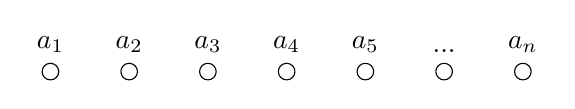
\begin{tikzpicture}
            \vertex (v1) at (0,0) [label=above:$a_1$]{};
            \vertex (v2) at (1,0) [label=above:$a_2$]{};
            \vertex (v3) at (2,0) [label=above:$a_3$]{};
            \vertex (v4) at (3,0) [label=above:$a_4$]{};
            \vertex (v4) at (4,0) [label=above:$a_5$]{};
            \vertex (v5) at (5,0) [label=above:$...$]{};
            \vertex (v6) at (6,0) [label=above:$a_n$]{};
            \path 
            ;
        \end{tikzpicture}

        The maximum number of topological order will be $n!$, where no tasks are dependant on another task (i.e. no edges).

        However, after a task is completed, the following task can only be a combination of the remaining tasks; therefore it is $n!$

        The minimum number of topological orders will be $1$ (with $n-1$ edges) , where every task is completed one after another.

        \[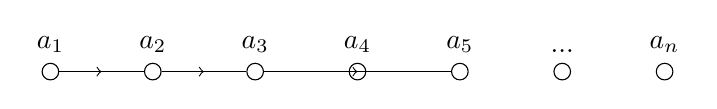
\begin{tikzpicture}[x=1.3cm, y=1cm,
            every edge/.style={
                draw,
                postaction={decorate,
                            decoration={markings,mark=at position 0.5 with {\arrow{>}}}
                           }
                }
        ]
            \vertex (v1) at (0,0) [label=above:$a_1$]{};
            \vertex (v2) at (1,0) [label=above:$a_2$]{};
            \vertex (v3) at (2,0) [label=above:$a_3$]{};
            \vertex (v4) at (3,0) [label=above:$a_4$]{};
            \vertex (v4) at (4,0) [label=above:$a_5$]{};
            \vertex (v5) at (5,0) [label=above:$...$]{};
            \vertex (v6) at (6,0) [label=above:$a_n$]{};
        \path
                (v1) edge (v2) 
                (v2) edge (v3)
                (v3) edge (v4)
            ;
        \end{tikzpicture}\]
        
    \end{homeworkProblem}

    \begin{homeworkProblem}
        \textbf{Question:} What is the maximal number of edges a directed graph with $n$ vertices can have? What is the maximal number of edges an undirected graph with $n$ vertices can have? Explain your answer.

        \textbf{Solution:} If we consider an edge, it is defined by its start vertex and its end vertex. Since there are $n$ choices for the starting vertex, and since we assume there are no self loops there are $n-1$ choices for the end vertex.

        Thus for a directed graph (with no self edges) we have $n(n-1)$ edges. If there is however self edges then the answer is simply $n^2$.

        If we have an undirected graph (we do not take into consideration self loops). And since we do not consider direction for an undirected graph $\{a,b\}$ implies $a \to b$ and $b \to a$ then there will half as much edges in an undirected graph. Therefore there will be $\frac{n(n-1)}{2}$ edges.
    \end{homeworkProblem}

    \begin{homeworkProblem}
        \textbf{Question:} Give example of $3n$ requests such that the solution based on “select the smallest interval” gives n requests, while an optimal solution consists of $2n$ intervals. You can explain your answer by drawing your solution or by explicitly writing the intervals down.

        \textbf{Solution:} 

        Consider these requests at certain times:

        \begin{tikzpicture}
            \draw (0,0) -- (3,0)  node[above,xshift=-1.5cm] {$r_1$};
            \draw (2.6,-0.5) -- (3.7,-0.5) node[above,xshift=-0.55cm] {$r_2$};
            \draw (3.2,-1.0) -- (5.5,-1.0) node[above,xshift=-1.15cm] {$r_3$};
        \end{tikzpicture}

        If we choose to select by smallest interval, only $r_2$ is selected. However, the optimal solution will select $r_1$ and $r_3$ 
            
    \end{homeworkProblem}

    \begin{homeworkProblem}
        \textbf{Question:} Suppose the selection rule for the interval scheduling problem is the following. Select a request that has the fewest possible requests overlapping it. Give an example where this rule does not provide an optimal solution.

        \textbf{Solution:} 

        Consider these requests at certain times:

        \begin{tikzpicture}
            \draw (0,0) -- (2.8,0)  node[above,xshift=-1.4cm] {$r_1$};
            \draw (3.1,0) -- (5.9,0) node[above,xshift=-1.4cm] {$r_2$};
            \draw (6.2,0) -- (9,0) node[above,xshift=-1.4cm] {$r_3$};
            \draw (9.3,0) -- (12.1,0) node[above,xshift=-1.4cm] {$r_4$};
            \draw (2.4,-0.7) -- (3.4,-0.7) node[above,xshift=-0.5cm] {$r_5$};
            \draw (5.5,-0.7) -- (7.5,-0.7) node[above,xshift=-1cm] {$r_6$};
            \draw (8.5,-0.7) -- (10,-0.7) node[above,xshift=-0.75cm] {$r_7$};
            \draw (2.4,-1.4) -- (3.4,-1.4) node[above,xshift=-0.5cm] {$r_8$};
            \draw (8.47,-1.4) -- (9.97,-1.4) node[above,xshift=-0.75cm] {$r_9$};
            \draw (2.4,-2.1) -- (3.4,-2.1) node[above,xshift=-0.5cm] {$r_{11}$};
            \draw (8.5,-2.1) -- (10,-2.1) node[above,xshift=-0.75cm] {$r_{12}$};
        \end{tikzpicture}

        The greedy method suggested here accepts the middle request in the second row ($r_6$) and thereby ensures a solution of size no greater than three.

        However the optimal solution in this example is to accept the four requests in the top row. 



    \end{homeworkProblem}

    \begin{homeworkProblem}
        \textbf{Question:} For the interval scheduling problem consider the following rule to solve it. Always select the request, among available ones, with the latest starting time. Does this give an optimal solution to the problem? Explain your answer.

        \textbf{Solution:} Yes, the selection by latest starting time would provide optimal solution given that it also takes into account for no overlapping requests.
        The selection by earliest finishing time algorithm provides optimal solution as the resources will be available as soon as a request is satisfied therefore it
        maximizes the remaining time to process the rest of the requests. By flipping the start time and end time of all requests, repeating the process will give the same output as selecting
        by latest starting time, therefore it can also give an optimal solution.

        To prove the optimality of the schedule $S$ of the form $r_1 , r_2 , ..., r_n$ produced by
        selecting the latest starting time, we can compare it to an optimal schedule O of the
        form $r_1,r_2,...,r_k$ and prove that the cardinality of $S$ and $O$ and are the same. 
        
        Take the last requests from both schedules, $r_n$ and $r_k$ . By virtue of the algorithm, the following must be true 
        $s(r_n) \geq s(r_k)$ , meaning that $r_{k-1}$ must be compatible with $r_n$, as $r_{k-1}$ must be compatible with $r_k$

        This fact can be applied at every iteration. Meaning that if $k>n$ then there is a request $r_{k-n-1}$ that is compatible with $r_n$. But we know that the algorithm
        adds every compatible request, so the schedule produced by the algorithm must have the same cardinality of the optimal schedule.
    



    \end{homeworkProblem}

    \end{document}
    